\chapter{IRK: Puntu-Finkoa.}

\section{Sarrera.}


Puntu-finkoan oinarritutako \emph{non-stiff} sistema Hamiltondarren zenbakizko integraziotarako IRK metodoaren inplementazioa proposatuko dugu. Zientzian, konputazioak koma-higikorreko aritmetikarekin egien direnez, biribiltze erroreak soluzioen doitasuna mugatzen du. Hortaz, inplementazioa epe luzeko doitasun altuko zenbakizko integrazioetarako aplikagarria izateko, biribiltze errorearen eraginak txikia izan behar du. Era berean, integrazioan zehar biribiltze errorearen estimazioa ezagutzea interesgarria da. 

Integrazioaren exekuzio denborak onargarriak izan daitezen , honako aurrebaldintza finkatu dugu: ekuazio diferentzialaren eskuin aldeko funtzioaren sarrera eta irteera argumentuak makina zenbakiak izatea, hau da, konputagailuan hardware bidezko exekuzioa (azkarra) duen koma-higikorreko aritmetika erabiltzea. Gaur-egun, zientzia-konputazioan $64$-biteko koma-higikorreko aritmetikarekin (\emph{double} datu-mota) lan egiten da eta beraz, praktikan erabiltzaileak ekuazio diferentziala datu-mota honetan zehaztuko duela suposatuko dugu. 
 
Lehenengo Hairer-en inplementazioa  \cite{Hairer2008} aztertuko dugu. Ondoren, IRK inplementazioa hobetzeko gure proposamenak azalduko ditugu. Azkenik, zenbakizko gure inplementazioaren emaitzak erakutsiko ditugu.

\section{Hairer-en inplementazioa.}

Gure abiapuntua, Haier-ek \cite{Hairer2008} proposatutako inplementazio hartu dugu.  
Lan honetan, IRK metodo sinplektikoaren puntu-finkoaren inplementazio estandarrean biribiltze errorearen garapen okerraz jabetu ziren eta gainera, metodo sinplektiko esplizituetan agertzen ez zena. Hauen ustez, bi ziren errore honen jatorriak:

\begin{enumerate}
\item Integrazioan $a_{ij}, b_i \in \mathbb{R}$ koefiziente zehatzak erabili ordez, biribildutako $\tilde a_{ij},\tilde b_i \in \mathbb{F}$ erabiltzeak, aplikatutako IRK metodoa zehazki sinpletikoa ez izatea eragiten du.
\item Puntu-finkoaren geratze irizpide estandarra dela eta, urrats bakoitzean errore sistematikoa gertatzen da.
\begin{equation*}
\triangle ^{[k]} = \max_{i=1,\dots,s}\|Y_i^{[k]}-Y_i^{[k-1]}\|_{\infty} \le \delta
\end{equation*}

\end{enumerate}    

\paragraph*{}Arrazoi hauek aztertu ondoren, honako konponbideak proposatu zituzten:

\begin{enumerate}
\item Doitasun handiagoko koefizienteak erabili, hauetako bakoitza bi koma-higikorreko koefizienteen batura kontsideratuz,
\begin{equation*}
a_{ij}= a^{\ast}_{ij}+\tilde a_{ij}, \ b_i= b^{\ast}_i+\tilde b_i
\end{equation*} 
non $a^{\ast}_{ij}>\tilde a_{ij}$ eta  $b^{\ast}_i>\tilde b_i$ diren. 


\paragraph*{}Zehazki era honetan kalkulatu daitezke,
\begin{equation*}
a^{\ast}_{ij}=(a_{ij} \otimes 2^{10}) \oslash 2^{10},\ \ \tilde a_{ij}= a_{ij}\ominus a^{\ast}_{ij}.
\end{equation*}


\item Iterazioak geratu, definitutako norma txikitzeari uzten dionean.
\begin{equation*}
\triangle^{[k]} = 0 \ \ or \  \triangle^{[k]} \geqslant \triangle^{[k-1]}.
\end{equation*}
  	 	
\end{enumerate}

Hairer-ek bere \emph{Fortran} inplementazioa eskuragarri du (\href{http://www.unige.ch/~hairer/preprints.html}{Fortran kodea}). Jarraian Hairer-en algoritmoa laburtu dugu (alg.\ref{alg:Hairer-IRK}). Aipatutako hobekuntzaz gain, batura konpensatua erabiltzen duela azpimarratu nahi dugu (notazioa sinplifikatze aldera $Y_{n,i}$ gaiaren ordez, $Y_i$ adierazpena erabiliko dugu).
 

\begin{algorithm}[h!]
 \BlankLine
  $e=0$\;
  \For{$n\leftarrow 0$ \KwTo ($endstep-1$)}
  {
   \BlankLine
   $k=0$\;
   $Y_{i}^{[0]}=y_n+h \ c_i \ f(y_n) $\; 
   \BlankLine
   \While{ ($\triangle^{[k]} \ != 0 \ \ and \  \triangle^{[k]} < \triangle^{[k-1]}) $}
   {
    \BlankLine 
    $k=k+1$\;
    $F_{i}^{[k]}=f(Y_{i}^{[k-1]}) $\;
    $Y_{i}^{[k]}=y_n+ h \ \big(\sum\limits_{j=1}^{s} a^{\ast}_{ij} F_{j}^{[k]} \big) 
                          + h \ \big(\sum\limits_{j=1}^{s} \tilde a_{ij} F_{j}^{[k]} \big)$\; 
    $\triangle ^{[k]} = \max_{i=1,\dots,s}\|Y_{i}^{[k]}-Y_{i}^{[k-1]}\|_{\infty}$\;
   }
   \BlankLine
    $\delta^{\ast}_{n}=h \ \big(\sum\limits_{i=1}^{s} b^{\ast}_i F_{i}^{[k]} \big)$\;
    $\tilde{\delta}_{n}=h \big(\sum\limits_{i=1}^{s} \tilde b_i F_{i}^{[k]} \big)$\;
    $ee=\delta^{\ast}_{n}+e$\;
    $yy=y_n+ee$\;
    $ee=(y_n-yy)+ee$\;
    \BlankLine
    $ee=\tilde{\delta}_{n}+ee$\;
    $y_{n+1}=y_{n}+ee$\;
    $e=(yy-y_{n+1})+ee$\;            
   \BlankLine
 }
 \caption{Hairer IRK} \label{alg:Hairer-IRK}
\end{algorithm}


\section{Gure inplementazioa.}

IRK metodoaren puntu-finkoaren inplementazioan lau proposamen berri egin ditugu. Lehen bi proposamenak  Hairer-ek bere lanean proposatutako konponbideen hobekuntzak dira. Batetik, IRK-ren birformulazio bat erabiliz, IRK metodoaren koma-higikorreko koefizienteak sinplektizidade baldintza zehazki betetzea lortuko dugu. Bestetik, geratze irizpidean arazo batzuk topatu ditugu eta arazo hauek gainditzen dituen geratze irizpide sendoagoa garatu dugu. Beste bi proposamenak dagokionez, bata batura-konpensatuari erlazionatuta dago eta bestea biribiltze errorea monitorizatzeko proposamena da.

Bestalde kapitulu honen bukaeran, interpolazio bidezko atalen hasieraketa azalduko dugu. Bukatzeko, gure algoritmoa azalduko dugu.  

\subsection{Metodoaren birformulazioa (1.proposamena).}

IRK metodoa definitzen duten $a_{ij},b_i$ koefizienteak, biribildutako $\tilde a_{ij},\tilde b_i \in \mathbb{F}$ ordezkatzerakoan, sinpletizide baldintza ez da beteko,
\begin{equation} \label{eq:61}
b_{i}a_{ij}+b_{j}a_{ji}-b_{i}b_{j}=0, \ \ 1 \leqslant i,j \leqslant s.
\end{equation}  
  
Arazo hau gainditzeko asmoarekin, IRK metodoa era honetan birformulatuko dugu,
\begin{align}
\label{eq:62}
Y_{n,i}&=y_n+ \sum\limits_{j=1}^{s} \mu_{ij} L_{n,j},  \ \ L_{n,i}=hb_if(Y_{n,i}), \ \ i=1,\dots,s,\\
y_{n+1}&=y_n+\sum\limits_{i=1}^{s} L_{n,i},
\end{align}
non 
\begin{equation*}
\mu_{ij}=a_{ij}/{b_j}, \ \ 1 \le i,j \le s.
\end{equation*}

Eta sinplekzidade baldintza modu honetan berridatziko dugu,
\begin{equation}
\mu_{ij}+\mu_{ji}-1=0, \ \ \ 1 \le i,j \le s.
\end{equation}

Formulazio berri honek  estandarrarekiko duen abantaila handiena , sinplektizidade baldintzan biderketarik agertzen ez denez,  baldintza hau betetzen duten $\tilde \mu_{ij} \in \mathbb{F}$ koefizienteak aurkitzeko bidea errazten zaigula da. Honako izango da koefiziente hauek finkatzeko bidea:

\begin{enumerate}
\item $\mu_{ij}$ koefizienteak.

Batetik $s$-ataleko Gauss metodoetan, diagonaleko koefizienteek ($\tilde{\mu}_{ii}:=1/2, \ i=1,\dots,s$) koma-higikorreko adierazpen zehatza dute.

Bestetik gainontzeko koefizienteak erabakitzeko, lehengo $\tilde{\mu}_{ij}:=fl(\mu_{ij}), \ 1 \le j < i \le s$ koefizienteak balioekin finkatuko ditugu. Eta bigarrenik, $\tilde{\mu}_{ji}:=1-\tilde{\mu}_{ij} , \ 1 \le j < i \le s$ koefizienteei balioa esleituko diegu;  $1/2 < |\mu_{ij}| <2$ denez, eta Sterbenz-en Teoremaren (ikus. \ref{eq:4311}) arabera  $1-\tilde{\mu}_{ij}$ koma-higikorreko adierazpen zehatza du. 

Beraz, hauek ditugu simplektizitate baldintza zehazki betetzen duten koma-higikorreko $\tilde{\mu}_{ij}\in \mathbb{F}$ koefizienteak.   
\begin{equation}
\tilde{\mu}=\left(\begin{array}{cccc}
    1/2       & 1-fl(\mu_{21}) & \dots & 1-fl(\mu_{s1})      \\
    fl(\mu_{21})      & 1/2    & \dots & 1-fl(\mu_{s2})      \\
    \vdots            & \ddots         &       & \vdots      \\
    fl(\mu_{s1})      & fl(\mu_{s2})   & \dots & 1/2          \\ 
     \end{array}\right)
\end{equation}

\item $b_{i}$ koefizienteak.

Gure inplementazioan, $hbi$ koefizienteak aurre-kalkulatuko ditugu. Batetik, koefiziente hauek simetrikoak direla eta bestetik, $\sum\limits_{i=1}^{s} hb_i=h$ berdintza bete behar dela kontutan hartuz,
\begin{eqnarray}
hb_1=hb_s:= h - \sum\limits_{i=2}^{s-1} hb_i
\end{eqnarray}

\item $y_{n+1}=y_n+\sum\limits_{i=1}^{s}L_{n,i}$ baturan, batugaien ordena.

Batugaien ordenak, batura errekurtsiboen emaitzaren doitasunean eragina du \cite{Higham2002}. Zenbaki positiboen batura dugunean, egokiena magnitude txikienetik handienerako batugaien ordena erabiltzea da. Horregatik, honako batura $y_{n+1}=y_n+\sum\limits_{i=1}^{s} hb_i f(Y_{n,i})$ irizpide honi jarraituz, $b_i$ koefizienteen txikienetik handieneko ordenaren arabera kalkulatuko dugu. 

\end{enumerate}

\subsection{Geratze irizpidea (2.proposamena).}

Ekuazio inplizituaren (\ref{eq:62}) soluzioaren hurbilpena lortzeko puntu-finkoko iterazioa era honetan definituko dugu. Iterazioaren abiapuntua $Y_i^{[0]}$  finkatu eta $k=1,2,\dots$ iterazioetarako $Y_i^{[k]}$ hurbilpenak lortu dagokigun geratze irizpidea bete arte.
%\begin{equation}
%L_i^{[k]}=hb_if(Y_i^{[k-1]}), \ \ Y_i^{[k]}=y_n+\sum\limits_{j=1}^{s} \mu_{ij} L_j^{[k]}
%\end{equation}

\begin{algorithm}[H]
 \For{ (k=1,2,\dots)}
  {
   $L_i^{[k]}=hb_if(Y_i^{[k-1]}) $\;
   $Y_i^{[k]}=y_n+\sum\limits_{j=1}^{s} \mu_{ij} L_j^{[k]} , \ \  i=1,\dots,s $\; 
   }
 \caption{Puntu-finkoko iterazioa.}
\end{algorithm}
 
\paragraph*{}IRK metodoaren inplementazio estandarrean geratze irizpidea honakoa da,
\begin{equation*}
\triangle^{[k]}=(Y_1^{[k]}-Y_1^{[k-1]},\dots,Y_s^{[k]}-Y_s^{[k-1]}) \in \mathbb{R}^{sd},
\end{equation*} 
\begin{equation}
\|\triangle^{[k]}\| \le tol
\end{equation}
non $\|.\|$ aurre-finkatutako bektore norma eta \emph{tol} tolerantzia errorea den . Tolerantzia txikiegia aukeratzen bada, gerta daiteke tolerantzia hori ez lortzea eta infinituki iterazioak exekutatzea. Baina tolerantzia ez bada behar adina txikia  aukeratzen, iterazioa puntu-finkora iritsi aurretik geratuko da eta lortutako $Y_i^{[k]}$ hurbilpenak biribiltze errorea baino errore handiago izango du.

Hairer-ek proposatu zuen geratze irizpidea gogoratuko dugu; $\triangle^{[k]} = 0$ (puntu-finkora iritsi delako) ;  edo   $\triangle^{[k]} \geqslant \triangle^{[k-1]}$ (biribiltze errorea nagusi delako). Orokorrean, geratze irizpide honek ondo funtzionatzen du baina esperimentalki zenbait kasuetan, iterazioak goizegi geratu direla konprobatu dugu. Gure iritziz, honen arrazoia da $\triangle^{[k]} \geqslant \triangle^{[k-1]}$ biribiltze errorea nagusia dela adierazten duen arren, badago $j \in \{1,\dots,sd\}$ osagairik,   $|\triangle_j^{[k]}| < |\triangle_j^{[k-1]}|$ hobetzeko tartea duena. 

Gure proposamena azaldutako arazoari soluzioa emateko, iterazioak jarraitzea honako baldintza betetzen den artean,
\begin{equation}
\exists j \in \{1,\dots,sd\} \ , \ |\triangle_j^{[1]}| >|\triangle_j^{[2]|}>\dots>|\triangle_j^{[k]}|>0.
\end{equation}


\subsection{Biribiltze errorea gutxitzeko teknikak (3.proposamena).}

Koma higikorreko aritmetika atalean (ikus \ref{sec:4.4}.atala) birbiltze errorea gutxitzeko bi teknika aipatu genituen: batura konpensatua eta biderketaren biribiltze errorea jasotzeko modua. Batetik, IRK metodoetan batura konpensatuaren aplikazio estandarra hobetzeko proposamena azalduko dugu eta bestetik, biderketaren biribiltze errorea nola aplikatu urratsaren gehikuntzan.   

\subsubsection*{Batura konpensatua.}
Integrazioaren zenbakizko soluzioa  $y_{n+1} \approx y(t_{n+1})$  lortzeko, urrats bakoitzean honako batura dugu,
\begin{equation*}
y_{n+1}=y_{n} + \phi(y_{n,h}), \ \ n=0,1,2,\dots.
\end{equation*}   

IRK metodoetan, $\phi: \mathbb{R}^{[d+1]} \rightarrow \mathbb{R}^d$ gehikuntza,
\begin{equation*}
\phi(y_{n,h})=\sum\limits_{i=1}^{s} L_{n,i},
\end{equation*}
non $L_{n,i}$ ($i=1,\dots,s$) inplizituki definitzen den.

\paragraph*{}Urrats askotako integrazioetan, batura honetan gertatutako biribiltze erroreak doitasun galera garrantzitsua sortzen du. Beraz, zenbakizko integrazioetan biribiltze errorea gutxitzeko  batura konpensatu estandarra aplikatzea oso erabilgarria zaigu (ikus \ref{alg:71} algoritmoa).

\begin{algorithm}[h]
 \BlankLine
  ${e}_{0}=0$\;
  \BlankLine
  \For{$n\leftarrow 0$ \KwTo ($endstep-1$)}
  {
   Hasieratu  $Y_{n,i}^{[0]} \ \ , \ \ i=1,\dots,s $\;
   Puntu-finkoko-iterazioak ($y_n, Y_{n,i})$ \;
   \BlankLine
    ${\delta}_{n}= \big(\sum\limits_{i=1}^{s} L_{n,i}^{[k]}\big) +  {e}_{n} $\;
    ${y}_{n+1}={y}_{n} + {\delta}_n$\;
    ${e}_{n+1}=({y}_{n} - {y}_{n+1})+ {\delta}_n$\;            
   \BlankLine
 }
 \caption{Batura konpensatua estandarra.}
 \label{alg:71}
\end{algorithm}

$y_{n+1} \in \mathbb{R}^{d}$,  $y_{n+1}=\tilde y_{n}+\tilde \delta_n$ soluzioa zehatza izanik eta $\tilde y_{n+1} \in \mathbb{F}^{d}$,  $\tilde y_{n+1}=\tilde y_{n} \oplus \tilde \delta_n$ koma-higikorreko hurbilpena izanik, lortutako errore estimazioa $\tilde{e}_{n+1}$ ,  baturan egindako  biribiltze errorea zehatza da,
\begin{equation}
y_{n+1}=\tilde {y}_{n+1}+\tilde {e}_{n+1}. 
\end{equation}

Horregatik, IRK metodoaren inplementazioan, inplizituki $Y_{n,i}$ atalak askatzeko ekuazioetan, $\tilde {y}_n$ ordez ($\tilde{y}_n \oplus \tilde{e}_{n}$) erabiltzea proposatzen dugu, 
\begin{equation}
\label{eq:eqbk}
L_{n,i}^{[k]}=hb_if(Y_{n,i}^{[k-1]}), \ \ \ Y_{n,i}^{[k]}=\tilde{y}_n \oplus \big(\tilde{e}_{n} \oplus \sum\limits_{j=1}^{s} \mu_{ij} L_{n,j}^{[k]}\big).
\end{equation}

Aldaketa honekin, lortutako zenbakizko soluzioaren doitasuna batura konpensatu estandarrarekin baino pixka bat hobea dela ikusi dugu. 

\subsubsection*{Biderketaren biribiltze errorea.}

Urratsa emateko unean, $L{n,i}=hb_i \ f(Y_{n,i})$ biderketaren biribiltze errorea kalkulatuko dugu eta $e_{n-1}$ gaiari gehituko diogu. Biderketaren biribiltze errorea jasotzeko konputagailuaren \emph{Fused Multiply Add} (FMA) eragiketan oinarritutko gara. 

%\begin{algorithm}[h]
%   \BlankLine
%    $EL_{i}=hb_i \ f(Y_{n,i})-L_{n,i}, \ \ i=1,\dots,s$\;
%    $e=e+\sum\limits_{j=1}^{s}EL_{j}$\;
%    $\delta_{n}=\sum\limits_{i=1}^{s} L_{n,i}+e$\;
%    $y_{n+1}=y_{n}+ \delta_{n} $\;
%    $e=(y_{n}-y_{n+1})+\delta_n$\;
%   \BlankLine
% \caption{Algorithm}
%\end{algorithm}

\begin{algorithm}[h]
 \BlankLine
  ${e}_{0}=0$\;
  \BlankLine
  \For{$n\leftarrow 0$ \KwTo ($endstep-1$)}
  {
   Hasieratu  $Y_{n,i}^{[0]} \ \ , \ \ i=1,\dots,s $\;
   Puntu-finkoko-iterazioak ($y_n, Y_{n,i})$ \;
   \BlankLine
    $EL_{i}=hb_i \ f(Y^{[k-1]}_{n,i}) - L^{[k]}_{n,i} \ \ , \ \ i=1,\dots,s$\;
    ${e}_{n}={e}_{n} + \sum\limits_{j=1}^{s}EL_{j}$\;
    ${\delta}_{n}= \big(\sum\limits_{i=1}^{s} L_{n,i}^{[k]}\big) + {e}_{n} $\;
    ${y}_{n+1}={y}_{n} + {\delta}_n$\;
    ${e}_{n+1}=({y}_{n} - {y}_{n+1})+ {\delta}_n$\;            
   \BlankLine
 }
 \caption{Biderketaren biribiltze errorea eta batura konpensatua.}
\end{algorithm}

\subsection{Biribiltze errorearen estimazioa (4.proposamena).}

Zenbakizko integrazioaren biribiltze errorearen estimazioa, bigarren zenbakizko integrazio baten soluzioaren diferentzia gisa kalkulatuko dugu. Bigarren integrazio honetan, $\delta_{n}$ gehikuntza mantisa txikiagoko zenbakira biribilduko dugu eta  horrela doitasun gutxiagoko soluzioa lortuz. 

$r\ge0$ zenbaki osoa, eta $x \in \mathbb{F}$ ($m$-bit doitasuneko koma-higikorreko zenbakia) izanik, honako funtzioa definituko dugu,

\begin{algorithm}[H]
  \SetAlgoLined\DontPrintSemicolon
  \SetKwFunction{algo}{algo}\SetKwFunction{floatR}{floatR}
  \SetKwProg{myalg}{Algorithm}{}{}
  \SetKwProg{myproc}{Function}{}{}
  \myproc{\floatR {x,r}}{
    $res=(2^r x + x)- 2^r x$\;
    \KwRet res \;}
  \caption{floatR}
\end{algorithm} 

\paragraph*{}Funtzio honek itzultzen duen balioa, $(m-r)$-bit doitasuneko koma-higikorreko zenbakia da. Beste modu batera esanda, $m$ biteko koma-higikorreko $x$ zenbakiaren azken $r$ bitak zeroan jartzen dituen funtzioa da.

 $r<m$ zenbaki osoa finkatuta, bigarren integrazioaren urratsa honela kalkulatuko dugu,
%\begin{equation}
%L_i^{[k]}=hb_if(Y_i^{[k-1]}), \ \ Y_i^{[k]}=floatR\bigg(\tilde{y}_n %\oplus \big(\tilde{e}_n \oplus \sum\limits_{j=1}^{s} \mu_{ij} %L_j^{[k]}\big),r\bigg).
%\end{equation}

%\begin{algorithm}[h]
%   \BlankLine
%    $\delta_{n}=floatR(\sum\limits_{i=1}^{s} L_{n,i}+e,r)$\;
%    $y_{n+1}=y_{n}+ \delta_{n} $\;
%    $e=(y_{n}-y_{n+1})+\delta_n$\;
%   \BlankLine
% \caption{Algorithm}
%\end{algorithm}


\begin{algorithm}[h]
\label{alg:71}
 \BlankLine
  $\hat{e}_{0}=0$\;
  \BlankLine
  \For{$n\leftarrow 0$ \KwTo ($endstep-1$)}
  {
   $\dots$\;
   \BlankLine
    $\hat{\delta}_{n}= floatR((\sum\limits_{i=1}^{s} L_{n,i}^{[k]}) \oplus \hat{e}_{n},r) $\;
    $\hat{y}_{n+1}=\hat{y}_{n} + \hat{\delta}_n$\;
    $\hat{e}_{n+1}=(\hat{y}_{n} -\hat{y}_{n+1})+ \hat{\delta}_n$\;            
   \BlankLine
 }
 \caption{Batura konpensatua estandarra.}
\end{algorithm}

Biribiltze errorearen estimazioa, zenbakizko soluzio nagusiaren $(y_n+e_{n})$ eta $r$ balio txiki baterako (adibidez $r=3$) kalkulatutako bigarren zenbakizko soluzioaren $(\tilde{\tilde{y}}_n+\tilde{\tilde{e}}_{n})$ arteko diferentziaren norma bezala kalkulatuko dugu. 
\begin{equation}
estimazioa_n=\|(y_n+e_{n})-(\tilde{\tilde{y}}_n+\tilde{\tilde{e}}_{n})\|_2
\end{equation}

Gure algoritmoan estimazioa zuzenean lortzeko, bi integrazioak sekuentzialki modu eraginkorrean kalkulatuko ditugu. Urrats bakoitzean, bi integrazioen $Y_i,\tilde{\tilde{Y}}_i$ ($i=1,\dots,s$) ataletako balioak, biribiltze errorea estimazio handiegia ez den artean,  antzekoak mantentzen dira. Beraz, bigarren integrazioan iterazio kopuru txikia beharko dugu, lehen integrazioaren bukaerako $Y_i^{[k]}$ ($i=1,\dots,s$) atalen balioak, bigarren integrazioaren $\tilde{\tilde{Y}}_i^{[0]}$ (i = 1, . . . , s) atalen hasieratzeko erabiliz.  

\begin{algorithm}[h]
  \BlankLine
  \For{$n\leftarrow 0$ \KwTo ($endstep-1$)}
  {
    \BlankLine
    $Y_n^{[0]}=G(Y_{n-1},h)$\;
    $\dots$\;
    $y_{n+1}=y_{n}+\delta_n$\;
    ${e}_{n+1}=({y}_{n} - {y}_{n+1}) +{\delta}_n$\;       
    \BlankLine
    \BlankLine
    \eIf{$(initwithfirst)$}
    {$\tilde{\tilde{Y}}_{n}^{[0]}=Y_{n}^{[k]}+(\tilde{\tilde{y}}_n-y_n)$\;}
    {$\tilde{\tilde{Y}}_{n}^{[0]}=G(\tilde{\tilde{Y}}_{n-1},h)$\;}
    $\dots$\;
    $\tilde{\tilde{y}}_{n+1}=\tilde{\tilde{y}}_{n}+\tilde{\tilde{\delta}}_n$\;
    $\tilde{\tilde{e}}_{n+1}=(\tilde{\tilde{y}}_{n} - \tilde{\tilde{y}}_{n+1}) + \tilde{\tilde{\delta}}_n$\;
    \BlankLine
    \BlankLine
    $estimation_{n+1}=\|(y_{n+1}+e_{n+1})-(\tilde{\tilde{y}}_{n+1}-\tilde{\tilde{e}}_{n+1})\|_2$\;
    \BlankLine
   }
 \caption{RKG2: errore estimazioa}
\end{algorithm}

\subsection{Atalen hasieraketa.} 

Ideia da, aurreko urratseko $(t_{n-1}+hc_i,Y_{n-1,i}), \ i=1,\dots,s$ eta $(t_{n-1}+h,y_{n})$, uneetako balioei dagokien polinomio interpolatzailea erabiliz, urrats berriaren atalen hasieraketa  $(t_{n}+hc_i,Y_{n,i}^{[0]}), \ i=1,\dots,s$ kalkulatzea. 
\begin{figure}[h]
\centerline{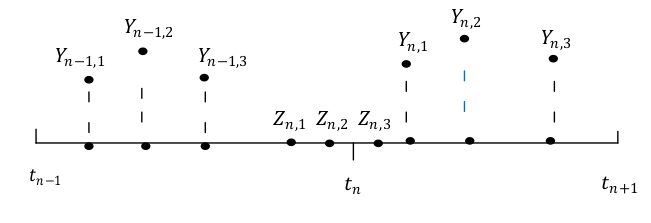
\includegraphics[width=12cm, height=4cm] {Interpolazioa}}
\caption{Interpolazioa.}
\label{fig:bost}
\end{figure}

\paragraph*{}($n-1$). urratseko informazioa erabiliz,
\begin{align*}
\left \{ \begin{array}{c}
Y_{n-1,i} =y_{n-1}+h \sum\limits_{j=1}^{s} a_{ij} f(Y_{n-1,j}),\\
y_n =y_{n-1}+h \sum\limits_{j=1}^{s} b_j f(Y_{n-1,j}),\\
\end{array} \right.
\ \Rightarrow \ \ 
Y_{n-1,i} &=y_n+h \sum\limits_{j=1}^{s} (a_{ij}-b_j) f(Y_{n-1,j}).
\end{align*}

Dagokion polinomio interpolatzailea,
\begin{equation*}
P(t)=  l_1(t) Y_{n-1,1}+\dots+l_s(t) Y_{n-1,s}+l_{s+1}(t) y_n
\end{equation*}
  
non $l_i(t)$ Lagrangiar polinomioa dugun,
\begin{equation*}
 l_i(t)=\prod_{l\neq i,l=1}^{s+1} \frac{(t-(t_{n-1}+hc_l))}{(c_i-c_l)}, \ \ c_{s+1}=1.
\end{equation*}

Eta beraz,
\begin{equation}
Y_{n,i} \approx Y_{n,i}^{[0]}= P(t_n+hc_i) = y_n+ h \sum\limits_{j=1}^{s} \lambda_{ij}f(Y_{n-1,j})
\end{equation}

\paragraph*{} Modu honetan s-ataletako IRK metodo bakoitzari dagokion $\lambda_{ij}$ koefiziente interpolatzaileak lortu daitezke. Polinomio interpolatzailearen bidezko hasieraketa ona izango da, emandako urratsa ez bada oso handia eta problema stiff ez denean. Era berean aipatu nahi genuke, atal askotako metodoetan (adibidez $s=16$)  interpolaziozko koefizienteen kalkuluan ezabapen arazoak,  doitasun handian lan egitea behartzen gaituela interpolaziozko hasieraketa ona izateko.  

\subsection{Algoritmoa.}

Formulazio berriari dagokion algoritmo orokorra,
%\begin{algorithm}[h]
% \BlankLine
%  $e_0=0$\;
%  \For{$n\leftarrow 0$ \KwTo ($endstep-1$)}
%  {
%   \BlankLine
%   Hasieratu  $Y_{n,i}^{[0]} \ \ , \ \ i=1,\dots,s $\;
%   \BlankLine
%   \While{ (konbergentzia lortu)}
%   {
%    \BlankLine 
%    $L_{n,i}=hb_if(Y_{n,i}) \ \ , \ \  i=1,\dots,s$\;
%    $Y_{n,i}=y_{n}+ \ \sum\limits_{j=1}^{s} \mu_{ij} L_{n,j}  \ \ , \ \  i=1,\dots,s$\;  
%   }
%   \BlankLine
%    $EL_{i}=hb_i \ f(Y_{n,i})-L_{n,i}, \ \ i=1,\dots,s$\;
%    $e_n=e_n+\sum\limits_{j=1}^{s}EL_{j}$\;
%    $\delta_{n}= \sum\limits_{i=1}^{s} L_{n,i}+e_n $\;
%    $y_{n+1}=y_{n}+ \delta_{n} $\;
%    $e_{n+1}=(y_{n}-y_{n+1})+\delta_n$\;
%   \BlankLine
% }
% \caption{Main Algorithm}
%\end{algorithm}

Eta puntu-finkoa erabiliz,

\begin{algorithm}[h]
 \BlankLine
  $e=0$\;
  \For{$n\leftarrow 0$ \KwTo ($endstep-1$)}
  {
   \BlankLine
   $k=0$\;
   Hasieratu  $Y_{n,i}^{[0]} \ \ , \ \ i=1,\dots,s $\;
   \BlankLine
   \While{ (konbergentzia lortu)}
   {
    \BlankLine 
    $k=k+1$\;
    $L_{n,i}^{[k]}=hb_if(Y_{n,i}^{[k-1]}) $\;
    $Y_{n.i}^{[k]}=y_{n} + \ \big(e+\sum\limits_{j=1}^{s} \mu_{ij} L_{n,j}^{[k]}\big)  $\;  
   }
   \BlankLine
    $EL_{i}=hb_i \ f(Y_{n,i})-L_{n,i}, \ \ i=1,\dots,s$\;
    $e=e+\sum\limits_{j=1}^{s}EL_{j}$\;
    $\delta_{n}= \sum\limits_{i=1}^{s} L_{n,i}^{[k]}+e $\;
    $y_{n+1}=y_{n}+ \delta_{n} $\;
    $e=(y_{n}-y_{n+1})+\delta_n$\;
   \BlankLine
 }
 \caption{IRK (puntu-finkoa).}
\end{algorithm}


\section{Esperimentuak.}


\subsection{Integrazio motak.}

Biribiltze erroreari dagokionez gure inplementazioa optimotik gertu dagoela erakutsi nahi dugu. Esperimentuetan lau integrazio mota egingo ditugu:

\begin{enumerate}

\item Koadruple doitasunezko ($128$-bit) integrazioa.

Zenbakizko integrazio hau soluzio zehatza kontsideratuko dugu eta errore globala kalkulatzeko erreferentziazko soluzioa izango da.

\item Integrazio ideala.

Koadruple doitasunezko integrazioa, ekuazio diferentzialaren eskuin aldeko funtzioaren ebaluazioa izan ezik. 
Ekuazio diferentziala double doitasunean ($64$-bit) definituko dela aurre baldintza harturik, integrazio ideala kontsideratuko dugu, hau da, hobetu ezin daitekeen integrazioa.    

\item Double doitasuna (batura konpensatu hobetua).

$64$-biteko koma higikorreko aritmetika eta \emph{batura konpensatua hobetua} erabiltzen duen inplementazioa, hau da,
atalen eguneraketan, ($\tilde{y}_n \oplus \tilde{e}_n$) (ekuazioa \ref{eq:eqbk}) espresioa erabilitako integrazioa.

\item Double doitasuna (batura konpensatu estandarra).

$64$-biteko koma higikorreko aritmetika eta \emph{batura konpensatu estandarra} erabiltzen duen inplementazioa (atalen eguneraketan $\tilde{e}_n$ gaia kontsideratzen ez duen integrazioa). 

\end{enumerate}

\subsection{Errore azterketa.}

Integrazio bakarra egin ordez, ausaz perturbatutako $P$ hasierako balio ezberdinetarako integrazioak exekutatu ditugu eta emaitza guzti hauen batazbestekoan oinarritu gara, biribiltze errorearen azterketa egokia egiteko.    

\subsubsection*{Adibidea.}

Ausazko perturbazioak kalkulatzeko funtzio bat definituta,
\begin{lstlisting} [language=Mathematica]
Pert[e0_,k_]:={e0*(k*RandomReal[{-1,1}])};
\end{lstlisting}

Perturbaziorik gabeko hasierako balioa $(u_0,e_0)$ eta $k$ perturbazio tamaina finkatuta, era honetan kalkulatuko dugu $(up_0,ep_0)$ perturbatutako hasierako balioa,
\begin{lstlisting} [language=Mathematica]
k = 2^35;
aux = Pert[e0, k];
up0 = N[u0] + aux;
aux2=up0-N[u0];
ep0=aux-aux2;
\end{lstlisting}


\subsubsection*{Notazioa.}  

$k$. integrazioan $N$ urrats eman baditugu, $t_i=t_0+i*h, \ i=1,\dots,N$ uneetarako lortuko dugu 
zenbakizko soluzioa,
\begin{equation*}
(q_i^{[k]},p_i^{[k]})\approx(q(t_i)^{[k]},p(t_i)^{[k]}), \ \ \ i=1,\dots,N.
\end{equation*}

\paragraph*{}Sistema Hamiltondarretan energia kontserbatzen da, energiaren definizioa hau izanik $H(q(t),p(t))=E(t)$,
\begin{equation*}
E_i^{[k]}=H(q_i^{[k]},p_i^{[k]})=konst, \ \ \ i=1,\dots,N.
\end{equation*}

\subsubsection*{Neurtzeko faktoreak.}

Energia eta kokapen erroreak honako faktoreen bidez neurtuko ditugu.

\begin{enumerate}

\item Energia errore globala.
%, \ \ i=1,\dots,N \ eta \ k=1,\dots,P.
\begin{align*}
\triangle E_i^{[k]} &=\frac{(E^{[k]}_i-E^{[k]}_0)}{E^{[k]}_0}, \ \ \ i=1,\dots,N \ eta \ k=1,\dots,P.\\
\bar{\triangle E_i} &=\frac{1}{P} \sum_{k=1}^{P} \triangle E_i^{[k]}, \ \  \sigma_i =\sqrt{\frac{1}{P} \sum_{k=1}^{P} (\triangle E_i^{[k]}-\bar{\triangle E_i})^2},\\
\bar{MaxE } &=\max_{i=1,\dots,N} |\bar{\triangle E_i}|.
\end{align*}  

\item Energia errore lokala.

$P$ integrazio guztietarako, bi urratsen arteko energia lokalaren batazbestekoa ($\mu$) eta desbiazio estarrada ($\sigma$).            
\begin{align*}
\blacktriangle E_i^{[k]} &=\frac{(E^{[k]}_i-E^{[k]}_{i-1})}{E^{[k]}_0},\ \ \ i=1,\dots,N \ eta \ k=1,\dots,P, \\
\bar{\mu} &= \frac{1}{N\cdot P} \bigg(\sum_{k=1}^{P} \sum_{i=1}^{N} {\blacktriangle E_i^{[k]}\bigg)}, \ \
\bar{\sigma} = \sqrt{\frac{1}{N\cdot P} \bigg(\sum_{k=1}^{P} \sum_{i=1}^{N} {(\blacktriangle E_i^{[k]}-\bar{\mu)}^2}\bigg)}          
\end{align*}
           
\item Kokapen errore globala.

Doitasun laukoitzean lortutako soluzioa, soluzio zehatza kontsideratuko dugu,           
\begin{equation*}
yexact^{[k]}_i=\hat{y}^{[k]}_i=(\hat{q}^{[k]}_i,\hat{p}^{[k]}_i).
\end{equation*}

eta $k.$ soluzioari dagokion kokapen errorea,          
\begin{align*}
Ge^{[k]}_i &=\|\hat{q}^{[k]}_i-q^{[k]}_i\|_2, \\
\bar{Ge_i}  &= (\frac{1}{P}\sum_{k=1}^{P} Ge^{[k]}_i) \ , \
                          \bar{MaxGe}=\max_{i=1,\dots,N} (\bar{Ge_i})
\end{align*}     
           
\item Puntu-finkoa lortutako urratsen batazbesteko portzentajea ($\bar{\triangle}0$).
           
$\triangle0^{[k]}$,  $k.$ integrazioan puntu-finkoa lortutako urratsen portzentaia izanik,           
\begin{equation*}
\bar{\triangle}0= \frac{1}{p}\sum_{k=1}^{P}\triangle0^{[k]}.
\end{equation*}
 
\item Kokapen errore estimazioa ($\bar{\mu Q_i}$ , $\bar{\sigma Q_i}$). 
            
Biribiltze errorearen estimazioaren gogoratuz, 
\begin{equation}
Est_i^{[k]}=\|(q_i^{[k]}+eq_{i}^{[k]})-(\tilde{\tilde{q}}_i^{[k]}+\tilde{\tilde{eq}}_{i}^{[k]})\|_2
\end{equation}
            
Errore estimazioaren kalitatea neurtzeko,
\begin{align} \label{eq:eq_Qi}
Q_i^{[k]} &=\log_{10} \bigg(\frac{Est^{[k]}_i}{Ge^{[k]}_i}\bigg),\\
\bar{\mu Q_i} &=\frac{1}{P}\sum_{k=1}^{p} Q_i^{[k]} \ , \ \ 
 \bar{\sigma Q_i}=\sqrt{\frac{1}{P}\sum_{k=1}^{P} (Q_i^{[k]}-\bar{\mu Q_i})^2}
\end{align}

\end{enumerate} 

\subsection{Integrazio parametroak.}

Hiru problemetarako esperimentuetan, integrazio parametroak bateratu ditugu. 

\begin{enumerate}

\item $s=6$ ataletako Gauss IRK metodoa aplikatu dugu.

\item Epe luzeko integrazioak aztertu ditugu.

\item Urratsa, trunkatze errorea biribiltze errorea baino txikiagoa izan dadin aukeratu dugu. 

\item Integrazio mota bakoitza $P=1.000$ perturbatutako hasierako balio ezberdinekin integratu dugu. Perturbazioen kalkulurako $k=2^35$ balioa finkatu dugu, hau da, $10^{-6}$ mailako perturbazioak aplikatu ditugu problema guztietarako.  

\item Kokapen errorearen estimazioaren kalkuluan, integrazio nagusian $rdigits1=0$ eta bigarren integrazioan $rdigits2=3$ balioak erabili ditugu.

\end{enumerate}


\subsection{Pendulu bikoitza ez-kaotikoa.}

Problema honetan zehazki erabilitako integrazio tartea eta urratsa hauek izan dira,
\begin{align*}
& t_0=0, \ \ t_{end}=2^{12}, \\
& h=2.^{-12}, \\
& sampling=2^7. 
\end{align*} 


\begin{table} [H]
\caption{Pendulu Bikoitza ez-kaotikoaren laburpena.}
\label{tab:2}       % Give a unique label
\begin{tabular}{c|c c c c c} 
 Integrazio Mota   &  $\bar{\triangle}0$  &  $\bar{MaxE}$ & $\bar{\mu}$  & $\bar{\sigma}$   & $\bar{MaxGe}$  \\
                           &   \%            &       &          &            &         \\
 \hline
                           &                 &         &       &           &          \\
 Koadruple                 &   $93.6$        &  $2e10^{-19}$  & $1e10^{-25}$  & $2e10^{-20}$  &      \\	    
 Ideala                    &   $98.3$        &  $7e10^{-16}$  & $6e10^{-19}$  & $2e10^{-17}$ &  $5e10^{-12}$\\
 Double                    &   $94.8$        &  $1e10^{-15}$  & $9e10^{-19}$  & $2e10^{-17}$ &  $7e10^{-12}$\\
\end{tabular}
\end{table}

\begin{figure}[!h]
\centering
\subfloat[Energi errorea.]{
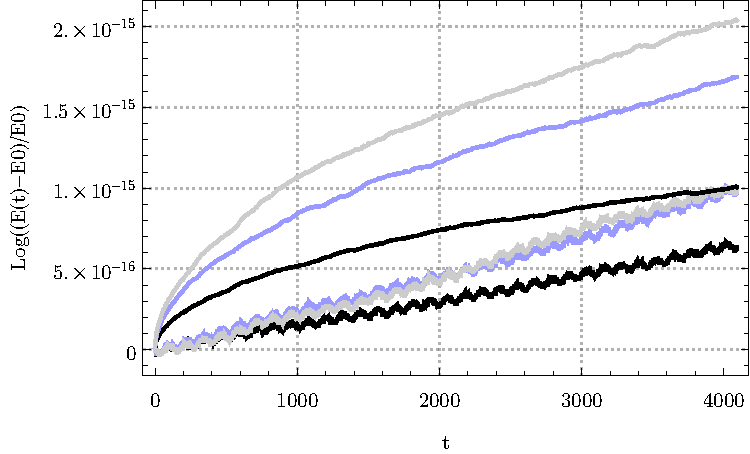
\includegraphics[width=.500\textwidth]{plot3a-2}
}
\subfloat[Kokapen errorea.]{
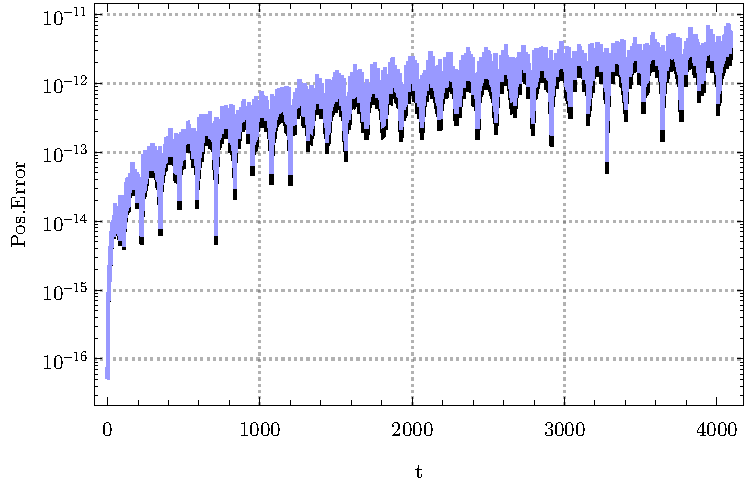
\includegraphics[width=.500\textwidth]{plot3b}
}
\caption[Pendulu-bikoitza: energi errorearen  eta kokapen errorearen eboluzioa.]
        {\small Pendulu-bikoitza ez-kaotikoa. Ezkerreko grafikoan,  energi errorearen batazbestekoa $\bar{\triangle E_i}$ eta desbiazio tipikoa $\sigma_i$ eboluzioa. Eskubiko grafikoan, kokapen errorearen eboluzioa $\bar{Ge_i}$. Integrazio ideala kolore beltzez, Double integrazioa (hobetua) kolore urdinez eta Double integrazioa (estandarra) gris kolorez.}
\label{fig:plot3}
\end{figure}        

\begin{figure}[!h]
\centering
\subfloat[Non-Chaotic: Ideal.]{
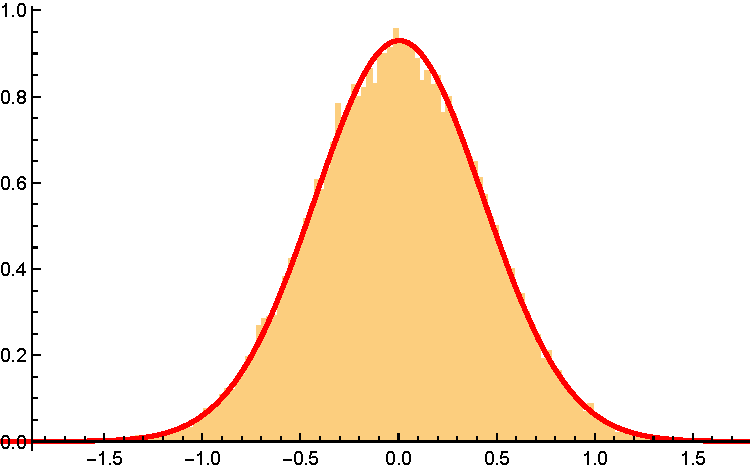
\includegraphics[width=.450\textwidth]{brouwer4a}
}
\subfloat[Non-Chaotic: rdigits=0.]{
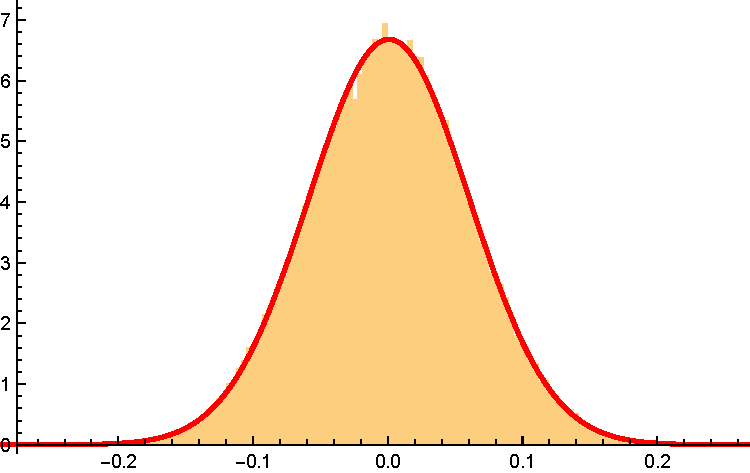
\includegraphics[width=.450\textwidth]{brouwer4b}
}
\caption{ \small Histogram of energy errors for Non-Chaotic case (a,b) and for Chaotic case (c,d).}
\label{fig:brouwer103}
\end{figure}


\begin{figure}[!h]
\centering
\subfloat[Non Chaotic: estimation]{
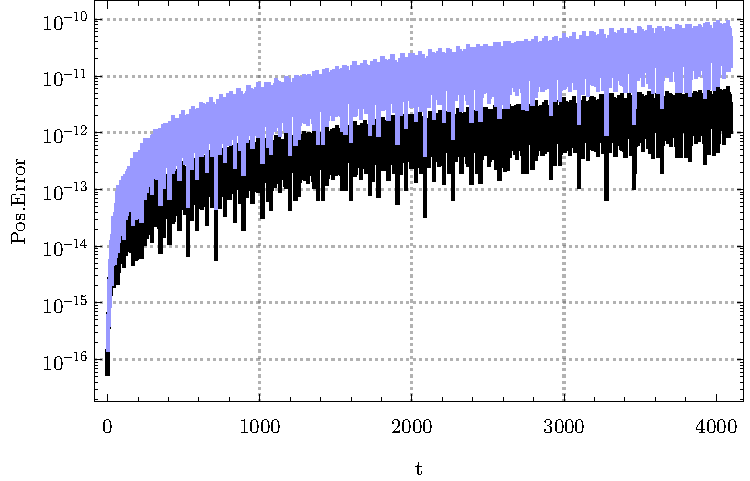
\includegraphics[width=.500\textwidth]{plot5a}
}
\subfloat[Non Chaotic: quality of estimation]{
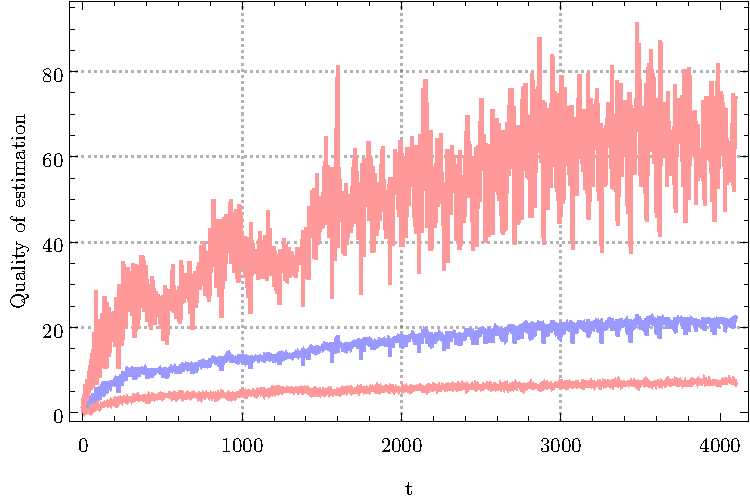
\includegraphics[width=.500\textwidth]{plot5b} 
}
\caption[Pendulu-bikoitza ez-kaotikoa: biribiltze errorearen estimazio.]

{\small Pendulu-bikoitza ez-kaotikoa: biribiltze errorearen estimazio. We compare evolution of our estimation error (blue) with evolution of global error (black). Estimation Quality. We show mean, $\bar{\mu Q_i}$ (blue) and  standard deviation, $\bar{\sigma Q_i}$ (red) of the quality according our definition of (\ref{eq:eq_Qi}).}
\label{fig:plotest}
\end{figure}

\clearpage
\subsection{Pendulu bikoitza kaotikoa.}

Problema honetan zehazki erabilitako integrazio tartea eta urratsa hauek izan dira,
\begin{align*}
& t_0=0, \ \ t_{end}=230, \\
& h=2.^{-12}, \\
& sampling=2^6. 
\end{align*} 


\begin{table} [h]
\caption{Summary of Chaotic case.}
\label{tab:3}       % Give a unique label
\begin{tabular}{c|c c c c c} 
 Arithmetic   &  $\bar{\triangle}0$  &  $\bar{MaxE}$ & $\bar{\mu}$  & $\bar{\sigma}$   & $\bar{MaxGe}$  \\
                           &   \%            &       &          &            &         \\
 \hline
                         &                 &         &       &             \\
 Quadruple prec          &   $93.6$        &  $2e10^{-19}$  & $7e10^{-22}$ & $1e10^{-20}$    &          \\	    
 Ideal Integrator        &   $98.3$        &  $3e10^{-16}$  & $1e10^{-18}$  & $9e10^{-18}$   & $0.18$    \\
 Double prec             &   $94.7$        &  $3e10^{-16}$  & $1e10^{-18}$  & $1e10^{-17}$   & $0.23$    \\
\end{tabular}
\end{table}


\subsubsection*{Energia eta kokapen erroreak.}


\subsubsection*{Brower legea.}

\begin{figure}[H]
\centering
\subfloat[Kaotikoa: Ideal.]{
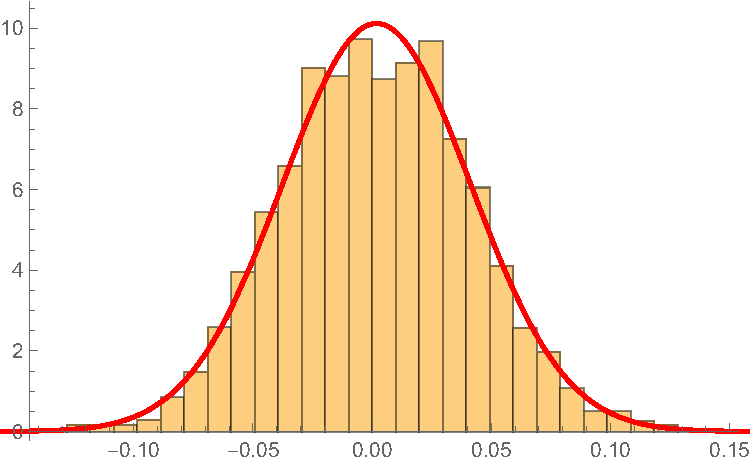
\includegraphics[width=.450\textwidth]{brouwer4c}
}
\subfloat[Kaotikoa: rdigits=0.]{
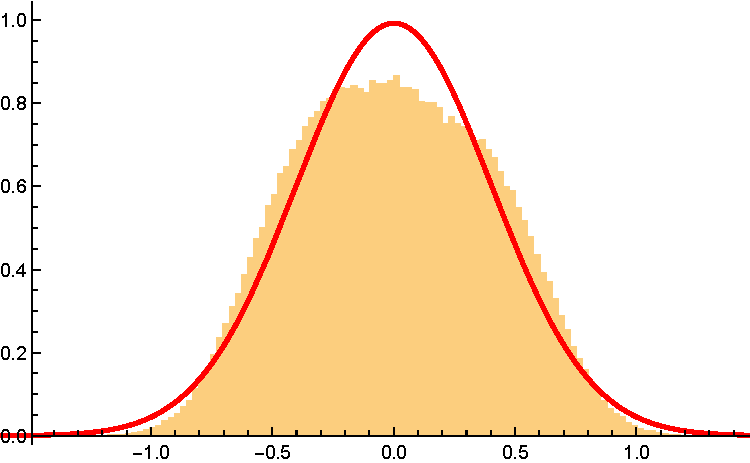
\includegraphics[width=.450\textwidth]{brouwer4d}
}
\caption{ \small Histogram of energy errors for Non-Chaotic case (a,b) and for Chaotic case (c,d).}
\label{fig:brouwer103}
\end{figure}

\subsubsection*{Errore estimazioa.}


\begin{figure}[h]
\centering
\subfloat[Non Chaotic: estimation]{
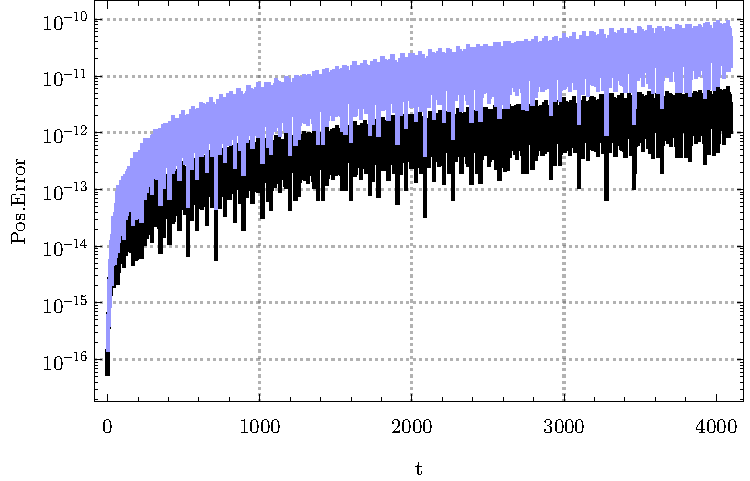
\includegraphics[width=.500\textwidth]{plot5a}
}
\subfloat[Non Chaotic: quality of estimation]{
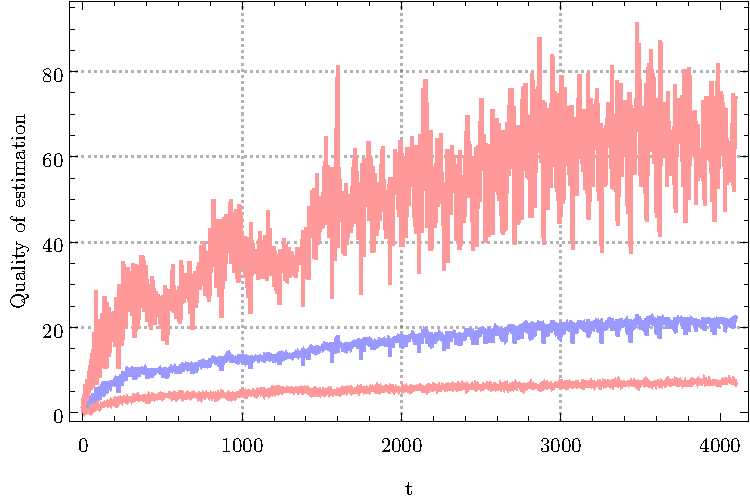
\includegraphics[width=.500\textwidth]{plot5b} 
}
\vskip\baselineskip
\subfloat[Chaotic: estimation]{
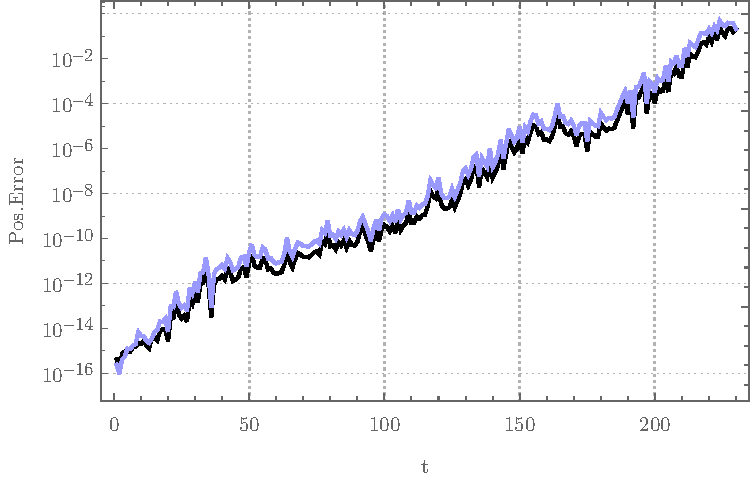
\includegraphics[width=.500\textwidth]{plot5c} 
}
\subfloat[Chaotic: quality of estimation]{
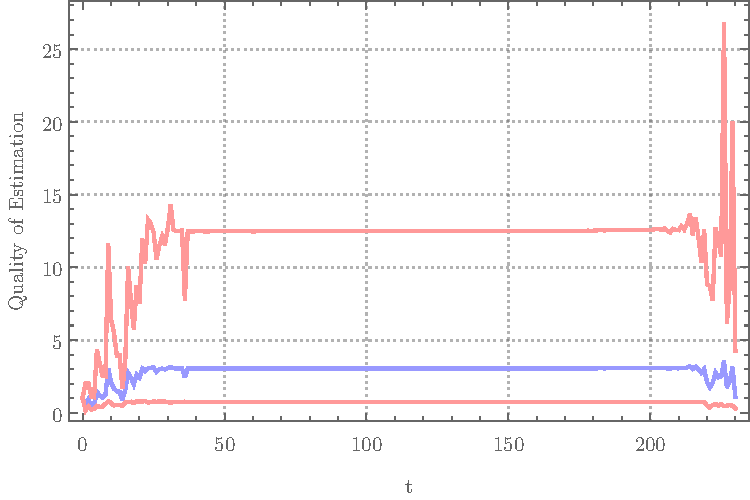
\includegraphics[width=.500\textwidth]{plot5d}
}

\caption[Pendulu-bikoitza: biribiltze errorearen estimazio.]{\small Estimation round-off error. We compare evolution of our estimation error (blue) with evolution of global error (black). Estimation Quality. We show mean (blue) and  standard deviation (red) of the quality according our definition of (\ref{eq:eq_Qi}).}
\label{fig:plotest}
\end{figure}

\clearpage
\subsection{N-Body problema.}


\begin{figure}[h]
\centering
\subfloat[Energy error.]{
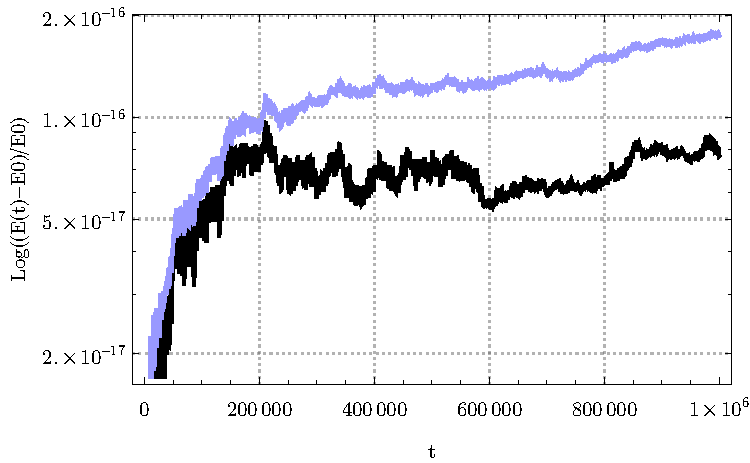
\includegraphics[width=.500\textwidth]{plot6a}
}
\subfloat[Global error.]{
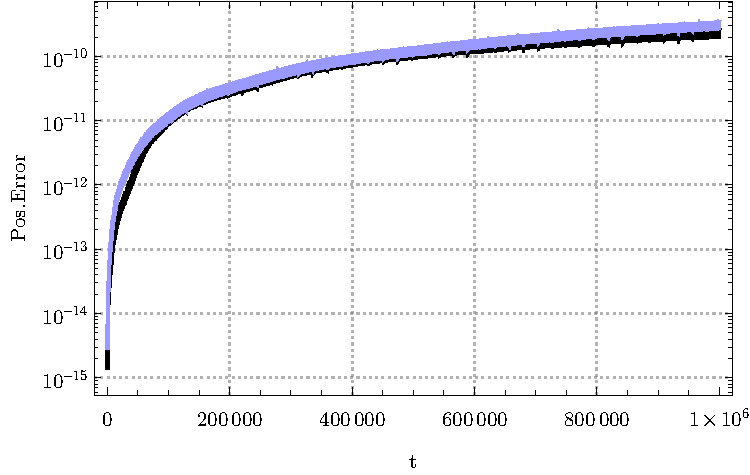
\includegraphics[width=.500\textwidth]{plot6b}
}
\caption[N-Body: energiaren errorearen eta errore globalaren eboluzioa.]{\small N-body: left figure mean energy error evolution $\bar{\triangle E_i}$ and right figure mean Global error evolution $\bar{Ge_i}$ of the 100 integrations for Ideal Integrator (black) and Double prec(blue).}
\label{fig:nbody1}
\end{figure}

\begin{figure}[h]
\centering
\subfloat[Estimation.]{
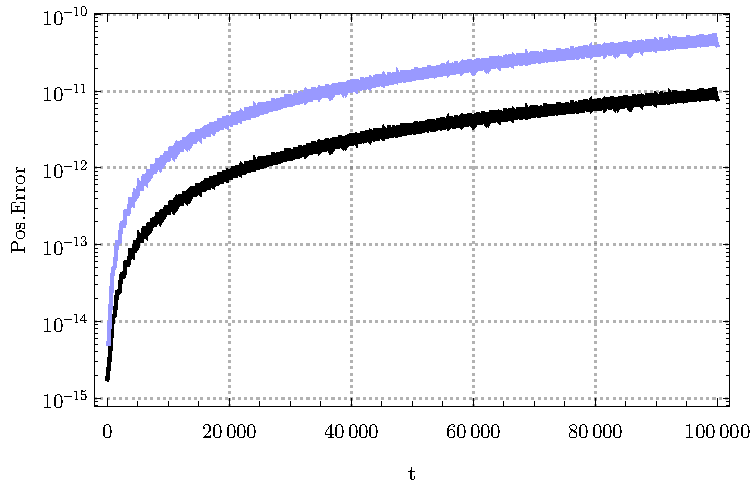
\includegraphics[width=.500\textwidth]{plot7a}
}
\subfloat[Quatlity.]{
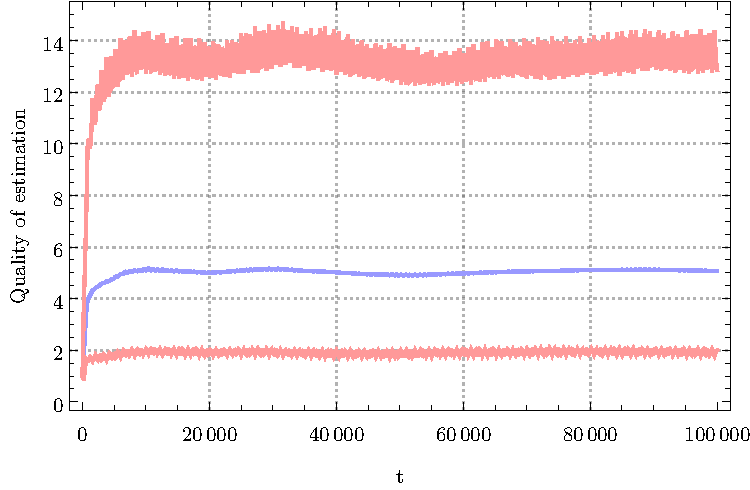
\includegraphics[width=.500\textwidth]{plot7b}
}
\caption[N-Body: birbiltze errorearen estimazioa.]{\small Left estimation round-off error, we compare evolution of our estimation error (blue) with evolution of global error (black). Right estimation Quality ,we show mean (blue) and  standard deviation (red) of the quality according our definition of (\ref{eq:eq_Qi}). We use rdigits1=0 and rdigits2=3.}
\label{fig:nbody2}
\end{figure}

\section{Laburpena.}
